\Author{\daAuthorTwo}

Since my research question "How can user-experience principals add to an intuitive map displayment for nonprofit activities in which people of different technical know-how levels collaborate?" is all about usability, I want to introduce you to its basic concepts and challenges but also provide some examples on how usability can impact a software's revenue and perception.

\blankLine

Usability is a critical aspect of software and interface design, ensuring that users can efficiently and effectively interact with a product or system. Its job is to provide clear feedback and "experiences" to the user, so interactions between software and human feel smooth and straight forward. Because each human being is different in its emotional experiences, it is difficult to design a kind of "one size fits all" solution. Due to this circumstance, many studies and experiments were conducted. \autocite{Paul:Usability101}

\subsection{Why it is important}

Usability ensures that users can accomplish their goals with minimal frustration and maximum efficiency. With the increasing reliance on digital tools, usability plays a key role, not only, in shaping user experiences but also accessibility of software for diverse user groups. A well-designed and thought-out usability concept can go a long way from refining a once tedious and complicated to use product, to one that can be operated even by non-familiar users or disabled people. This plays a big part in the inclusion of all age and knowledge groups as well as the general market share through mass adoption because of the easiness.

\subsection{Components of Usability}

According to Jakob Nielsen, usability consists of five core components. To achieve the best possible usability, each of factors must be taken into account and be improved to its maximum.

\begin{itemize}
    \item Learnability
    \begin{description}
        \item How \textbf{easy} it is to accomplish basic tasks the first time  
    \end{description}

    \item Efficiency
    \begin{description}
        \item How \textbf{quickly} task can be accomplished after an initial learning period
    \end{description}

    \item Memorability
    \begin{description}
        \item How \textbf{memorable} actions are to users so, after an extended period of not using a software
    \end{description}

    \item Error handling
    \begin{description}
        \item How \textbf{many} errors users make while using the design and how \textbf{sever} they are  
    \end{description}

    \item Satisfaction
    \begin{description}
        \item How \textbf{pleasant} the overall experience of using the product is 
    \end{description}
\end{itemize}
\autocite{Paul:Usability101}

\blankLine

Now that we are aware of these key points, what measures can we take to reach the goal of great usability? According to Nasrullah Hamidli, human-computer-interaction relies on consistency, visibility, feedback, and simplicity. Consistency ensures users do not need to learn new interactions for each task. For example, buttons should look alike and be in a similar location. This makes for a more natural navigation across the product and an overall familiar feel. Simplicity connects directly to this. Its goal is to minimize clutter and make user interfaces easy to understand and provide one, clear way to accomplish a task, not many possible, but complicated and unintuitive ways. It also aims to reduce distractions. Visibility allows users to clearly understand their options at any given moment, this is most often achieved through visual cues, like, grayed out buttons. This goes hand in hand with the feedback aspect, which provides immediate confirmation of actions. Loading indicators, color-changes and alike get used most often.

\blankLine

Another important part of designing a good UI are typography and colors. These
can act as parameters for the attention and emotions of users, as well as establish visual hierarchies, which intern, contribute again to a simpler to navigate interface. \autocite{Paul:UIUXIntroduction}

\subsection{Fundamental concepts}
In this section we will look further into these basic concepts and examine what designers can concretely do to improve usability. To make more descriptive, what impacts usability, we will, along the way, modify a simple website.

\blankLine

\begin{figure} [H]
    \center
    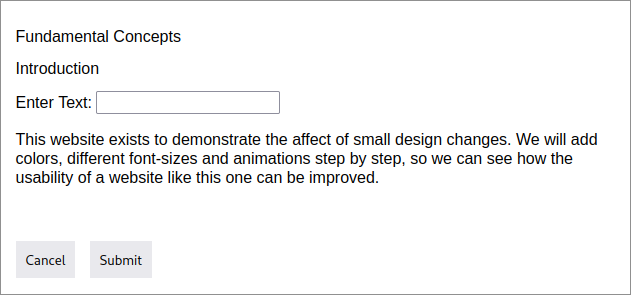
\includegraphics [width=0.9\textwidth] {images/paul/usabilityExamples/initialWebsite.png}
    \caption{Starting point of usability example website}
\end{figure}

\textbf{Visual Hierarchy}

Starting of with Visual hierarchy. It is the most basic principle in UI/UX design and dictates, how users perceive and navigate content. A strong visual hierarchy contributes to simplicity and ensures that important elements are more visually prominent, guiding users toward essential actions and information. Factors include the text size, weight and spacing. 

\blankLine

In the initial version, visitors of our website are not able to clearly and promptly differentiate between headings and actual text. This is due to the use of only a single font size and weight.


\blankLine

    If these attributes get tuned just a little, it becomes suddenly much easier to distinguish primary content from secondary information. Headings are bold and larger, while body text is appropriately sized for readability. Proper spacing and alignment create a structured and pleasant reading experience.
    
    \blankLine

    \begin{figure} [H]
        \center
        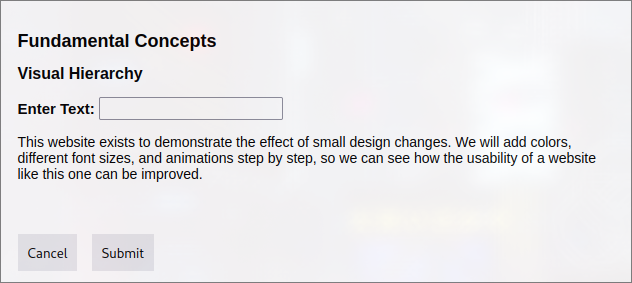
\includegraphics [width=0.9\textwidth] {images/paul/usabilityExamples/visualHierarchy.png}
        \caption{Example with better visual Hierarchy through different font size and weight}
    \end{figure}

\blankLine

\textbf{Color Theory \& Contrast}

Color selection plays a critical role in usability and aesthetics. Well-chosen colors draw the attention to important elements while poor color choices can make content inaccessible, especially for users with visual impairments. The advantages of attention through colors can also be used in reverse, for example, a button to delete something important may be colored red, to indicate a fatal action, but could also be gray, so the user must consciously decide to press it. This acts as a safety measure. 

\blankLine

To help designer with their color choices and visualize what colors work together, the color wheel was invented. On it, relations between colors can be shown easily. It consists of three groups of colors. 

\begin{itemize}
    \item \textbf{Primary}
    
    These are the fundamental colors that cannot be created by mixing other colors. They vary, depending on the media format they will be used on. On screens the \textit{RGB Model} is in use, while when printing color, cyan, magenta and yellow (CMY Model) get used.

    \item \textbf{Secondary}
    
    \textit{Secondary colors} arise by mixing two primary colors to equal amounts. In designing applications, they often get used for buttons or highlighting important information.

    \item \textbf{Tertiary}
    They are often associated with a calm and refined aesthetic. They are not quite the same eye-catchers as primary colors, rather they have their value in creating appealing combinations.
    
\end{itemize}

\begin{figure} [H]
    \center
    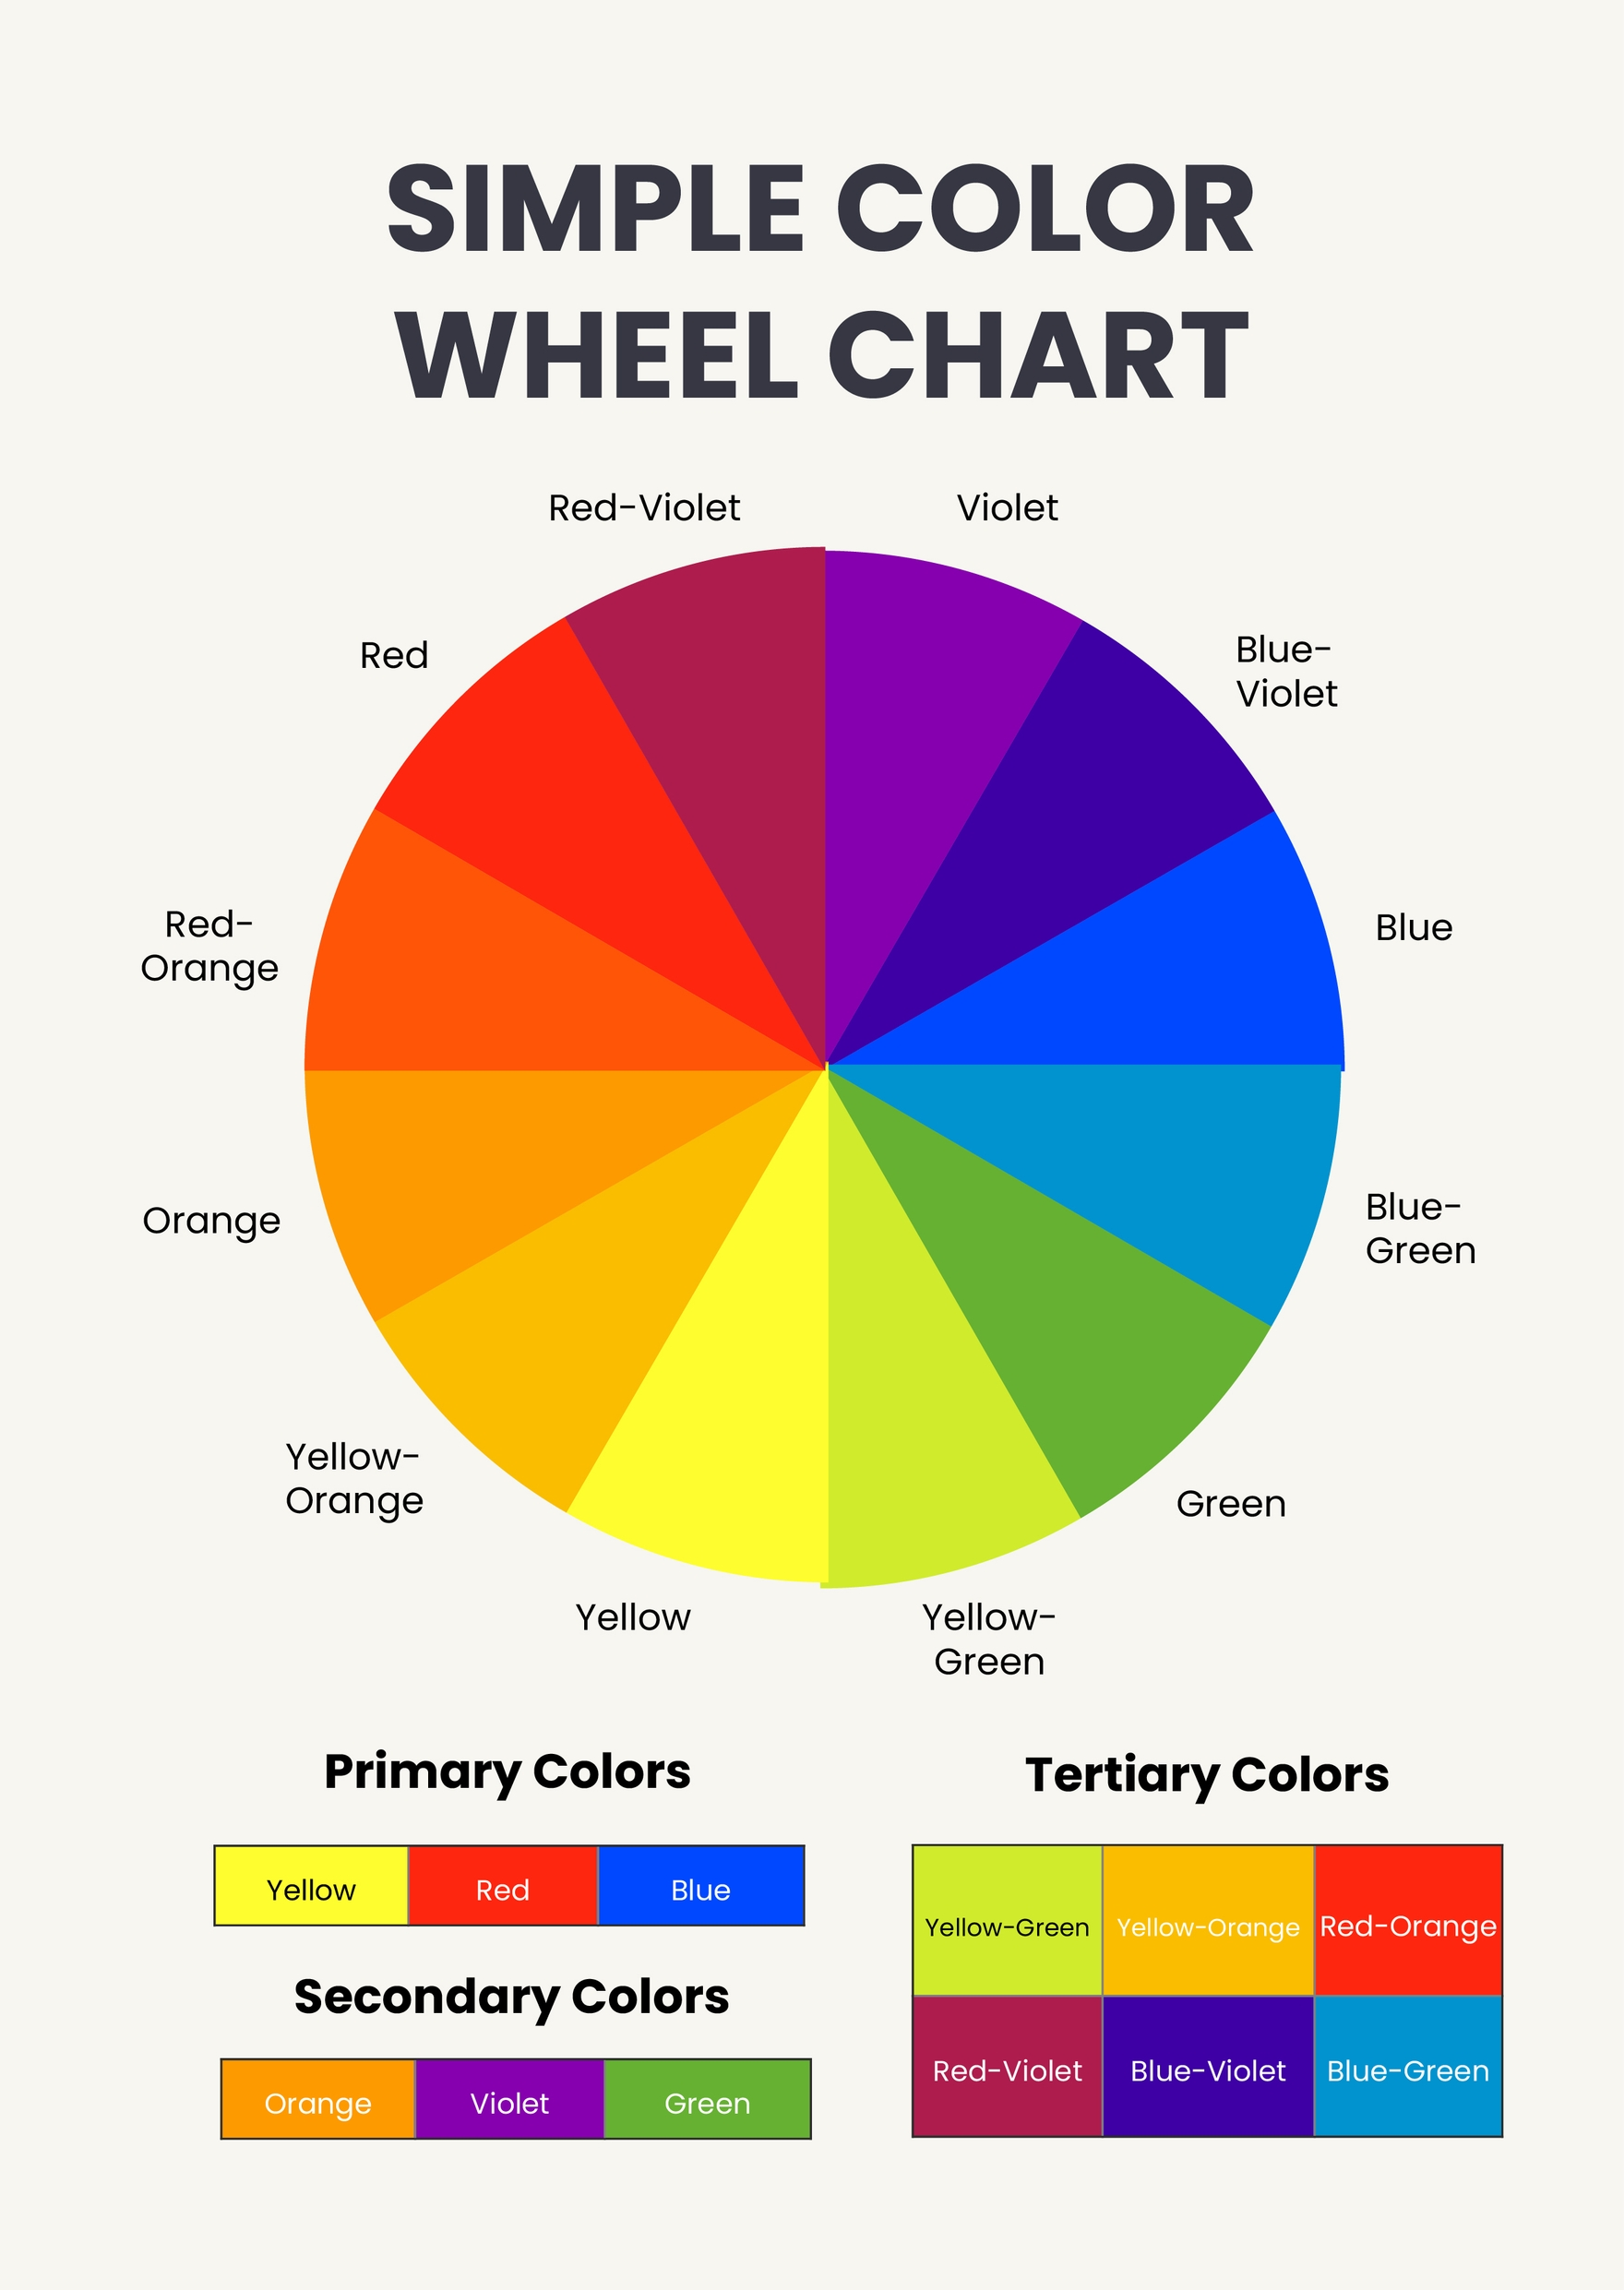
\includegraphics [width=0.5\textwidth] {images/paul/colorWheel.jpg}
    \caption{Color wheel with primary, secondary and tertiary colors sorted (Source: \url{https://www.template.net/editable/114132/simple-color-wheel-chart})}
\end{figure}

\begin{table} [H]
    \centering
    \begin{tabular} {|c|c|c|}
        \hline
        \multicolumn{1}{|c|}{\textbf{Relationship Type}} &
        \multicolumn{1}{c|}{\textbf{Description}}  &
        \multicolumn{1}{c|}{\textbf{Use case}}  \\
        
        \hline
        Complementary & Colors opposite each other & Creating bold contrast\\
        \hline
        Analogous & Colors next to each other & Harmonious, natural looks\\
        \hline
        Triadic & Three evenly spaced colors & Balanced, vibrant designs\\
        \hline
        Split Complementary & One color + two adjacent to its complement & Softer contrast than complementary\\
        \hline        
    \end{tabular}
    \caption{Key color combinations with effects(Source: \url{https://colorpage.ai/blog/color-theory-for-beginners})}
    \label{Table:ColorCombinations}
\end{table}

The current design doesn't feature any color at all. To highlight the buttons, we can give them a color. Now we also need to change the text color, because, if left as is, the contrast would not be great, and therefor the text harder to read. \autocite [vgl.]{Paul:ColorTheoryForBeginners}
    
    \begin{figure} [H]
        \center
        \includegraphics [width=0.9\textwidth] {images/paul/usabilityExamples/ColorTheoryExample.png}
        \caption{}
    \end{figure}

\blankLine

\textbf{Consistency}

Consistency in design enhances user experience by ensuring that UI elements and interactions are predictable across different states of the application. Also, a consistent aesthetic can create familiarity, brand recognition and improves the overall visual appeal.

\blankLine

\textbf{Button Placement \& Behavior}

Buttons are a critical and one of the most common interactive elements in UI design. Their placement, size and responsiveness affects usability and efficiency. Since the first graphical UIs, the actions to move forward were always on the right side. In contrast, actions to cancel are most commonly placed somewhere on the left. If designers choose to deliberately change this universal agreement, it leads to potential user errors. Also, a color-change on hover got implemented, so the user now gets clearly informed that all required fields are populated, and he can move on. 

\blankLine

    This design highlights the "Submit" Button, and places it in the correct location. Through this, the simplicity to use is improved because users do not have to search for the button that lets them continue. 
    
    \todo{Gendern?}

\blankLine

\textbf{Feedback}

Providing immediate and clear feedback enhances user confidence and prevents frustration. There are many forms in which such feedback can be provided, for example, vibrations, sounds or pop-up messages. Feedback can also be supplied by something like a grayed-out button, to signal that this action is not currently available. Success messages or error messages also add to the usability of a website, as well as loading indicators and different animations.


\blankLine

\subsection{Challenges in designing for a broad user spectrum}

Designing for a diverse user base requires the addressing of varying levels of experience, prior knowledge, cognitive abilities, and accessibility needs. Failure to account for these differences can lead to usability issues, preventing certain groups from effectively using a system. Designers must implement features such as adjustable text sizes, screen reader compatibility, and intuitive navigation to ensure accessibility for all users.

\blankLine

\todo{wenn zu wenig inhalt dann könnte man auch noch was schreiben wieso des so is und auf welchen psychologischen dingen des basiert}

Interfaces should always be tailored to the needs and expectations of the end-user. This leads to challenges when the user-group is not clearly defined or consists of people with widely different backgrounds. For example elderly people often need further guidance when interacting with digital solutions than members of younger generations. This leads back to the core components of usability-design, interfaces need to be simple and unmistakable in their functionality. Failing to provide these core concepts will sooner or later result in a frustrated and shrinking user base. 
\autocite{Paul:UIUXIntroduction}

\newpage